%&pdflatex
\documentclass[1p]{elsarticle}

\usepackage{lineno,hyperref}
\usepackage{amsmath, amssymb, amscd, amsthm, amsfonts}
\usepackage{mathtools}
\usepackage{xcolor}
\usepackage{lipsum}
\usepackage{tikz}

\DeclareMathAlphabet{\mathpzc}{OT1}{pzc}{m}{it}

\modulolinenumbers[5]

\setlength{\parskip}{.4em} 

\DeclarePairedDelimiter\ceil{\lceil}{\rceil} \DeclarePairedDelimiter\floor{\lfloor}{\rfloor}

\newtheorem{theorem}{Theorem}
\newtheorem{lemma}[theorem]{Lemma}
\newtheorem{conjecture}[theorem]{Conjecture}
\newtheorem{corollary}[theorem]{Corollary}
\newtheorem{example}[theorem]{Example}

\newcommand{\NPZ}{\ooalign{$Z$\cr\hfil\rule[.8ex]{.3em}{.09ex}\hfil\cr}}
\newcommand{\zn}{\ooalign{$z$\cr\hfil\rule[.5ex]{.2em}{.08ex}\hfil\cr}}
\newcommand{\sq}[1][black]{%
\begin{tikzpicture}                                                           
  \draw[#1] (2pt,0pt) -- (6pt,0pt);   
  \draw[#1] (2pt,0pt) -- (2pt,4pt);    
  \draw[#1] (2pt,4pt) -- (6pt,4pt);   
  \draw[#1] (6pt,0pt) -- (6pt,4pt);
  %\draw[white] (5pt,0pt) -- (6pt,0pt);                              
\end{tikzpicture}%
}                       
\newcommand{\sqSmall}[1][black]{%
\begin{tikzpicture}                                                           
  \draw[#1] (1.5pt,0pt) -- (4.5pt,0pt);   
  \draw[#1] (1.5pt,0pt) -- (1.5pt,3pt);    
  \draw[#1] (1.5pt,3pt) -- (4.5pt,3pt);   
  \draw[#1] (4.5pt,0pt) -- (4.5pt,3pt);
  %\draw[white] (5pt,0pt) -- (6pt,0pt);                              
\end{tikzpicture}%
}                       



\journal{Discrete Applied Mathematics}

\bibliographystyle{elsarticle-num}

\begin{document}

\section{An example for zombie number of Cartesian product of two graphs} \label{CartesianProductExample}
\begin{example} $\zn(P_3 \sq P_4 ) = 2$
\end{example}

\begin{figure}[h!]
	\centering
	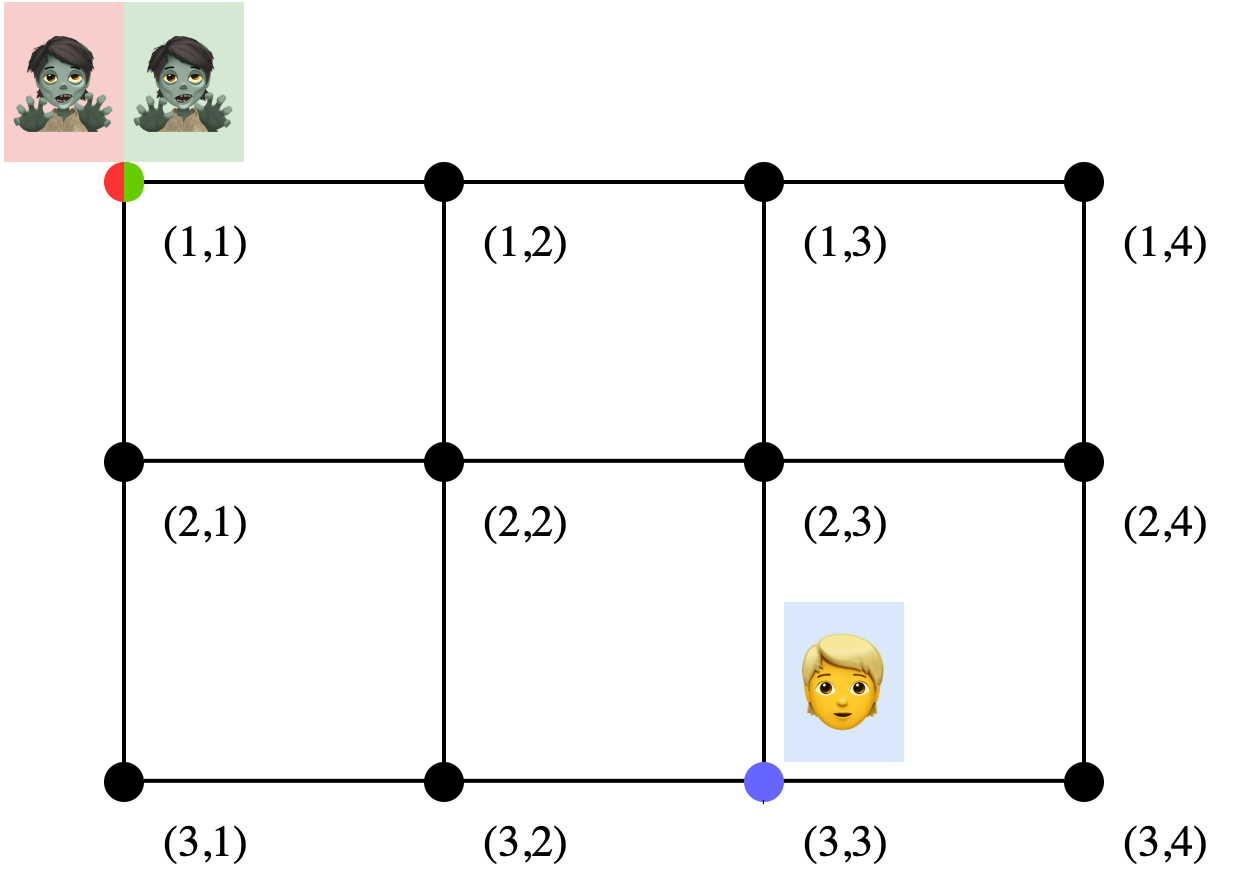
\includegraphics[width=0.5\linewidth]{p34m1.png}
	\caption{$P_3 \sqSmall P_4$ and initial vertices}
	\label{fig:p3}
\end{figure}

It is easy to show that $\zn(P_3) = \zn(P_4) = 1$. On each of these path graphs, zombie's initial position could be any
vertex of the graph. For this example, we put the {\it G-zombie} and {\it H-zombie} ($G = P_3$ and $H = P_4$) both on
vertex $(1,1)$. We show the survivor with blue color, {\it H-zombie} with red, and {\it G-zombie} with green. {\it
G-zombie} will try to get to the same $G_{i}$ as the survivor's which is $G_3$ using an {\it H-edge}. {\it H-zombie}
will try to get to $H_3$ (See figure \ref{fig:p4}).

\begin{figure}[h!]
	\centering
	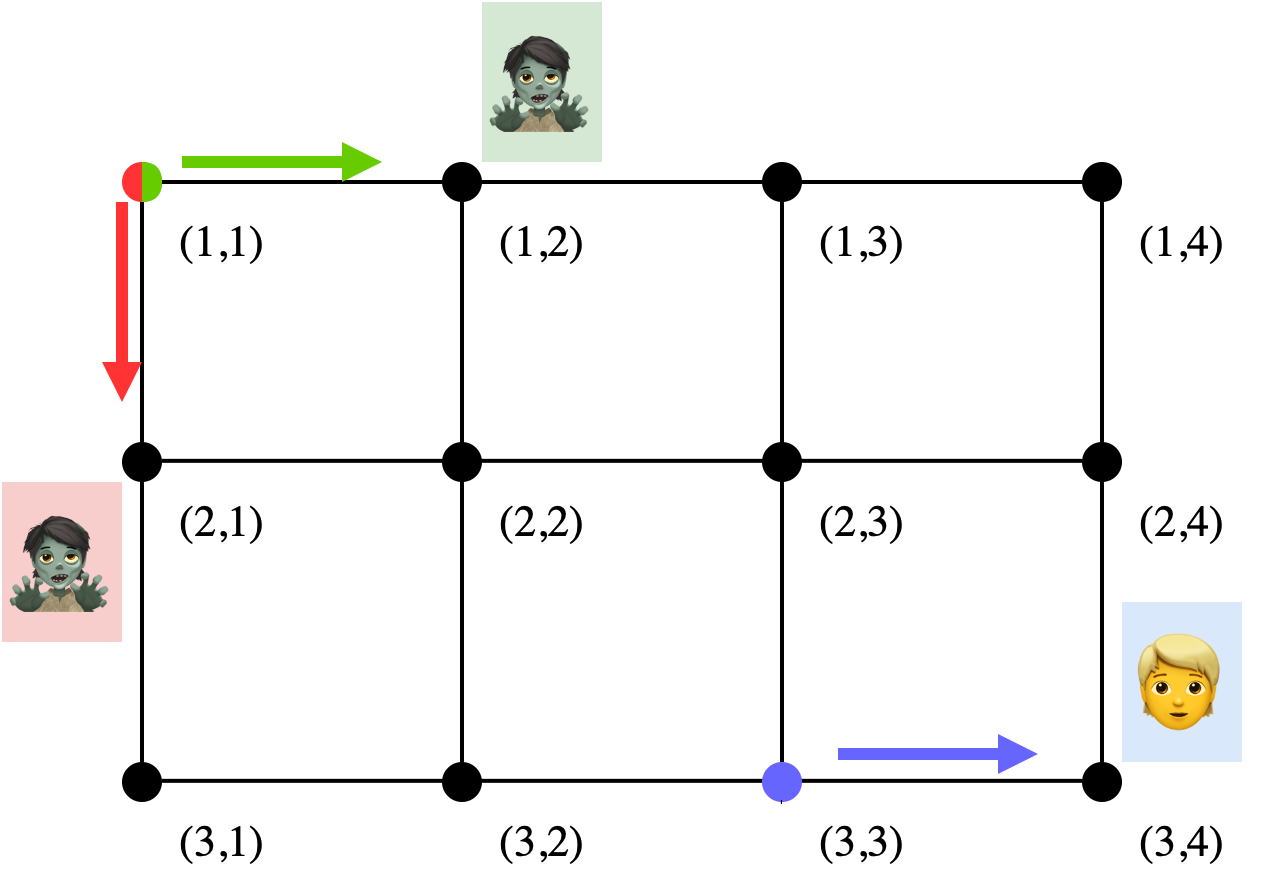
\includegraphics[width=0.5\linewidth]{p34m2.png}
	\caption{First move of players}
	\label{fig:p4}
\end{figure}

After zombies' move the survivor must move. No matter what move he makes, either {\it G-zombie} has made itself closer
to $H_x$ or {\it H-zombie} has made itself closer to $G_y$. In this case, {\it H-zombie} got closer to $H_x$. Since
neither {\it H or G-zombie}s share $H_x$ or $G_y$ with the survivor, they will still try to achieve that (See figure \ref{fig:p5}).

\begin{figure}[h!]
	\centering
	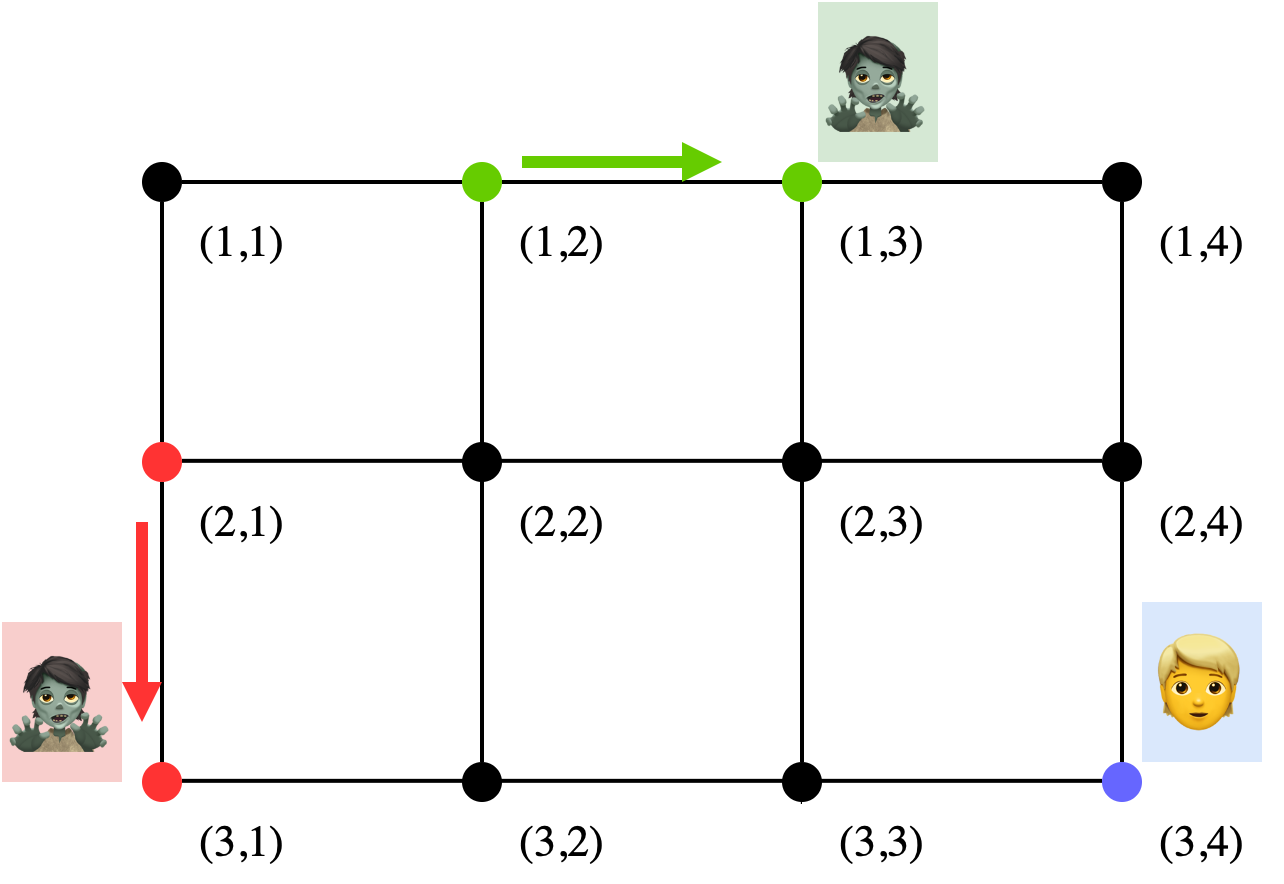
\includegraphics[width=0.5\linewidth]{p34m3.png}
	\caption{Second move made by zombies, third in total}
	\label{fig:p5}
\end{figure}

Now {\it H-zombie} shares the same copy of $H$ as the survivor and it is the survivor's turn. If the survivor moves to
another $H_i$, {\it H-zombie} will mimic the move. If the survivor makes an {\it H-move}, {\it H-zombie} will do
whatever it did on a single $H$ for capturing the survivor. This means the survivor cannot do infinite {\it H-move}s.
Thus for him being able to survive he has to do infinite {\it G-move}s, which again leads to {\it G-zombie} capturing
him. For other moves, you can see figure \ref{fig:p6}.

\begin{figure}[h!]
	\centering
	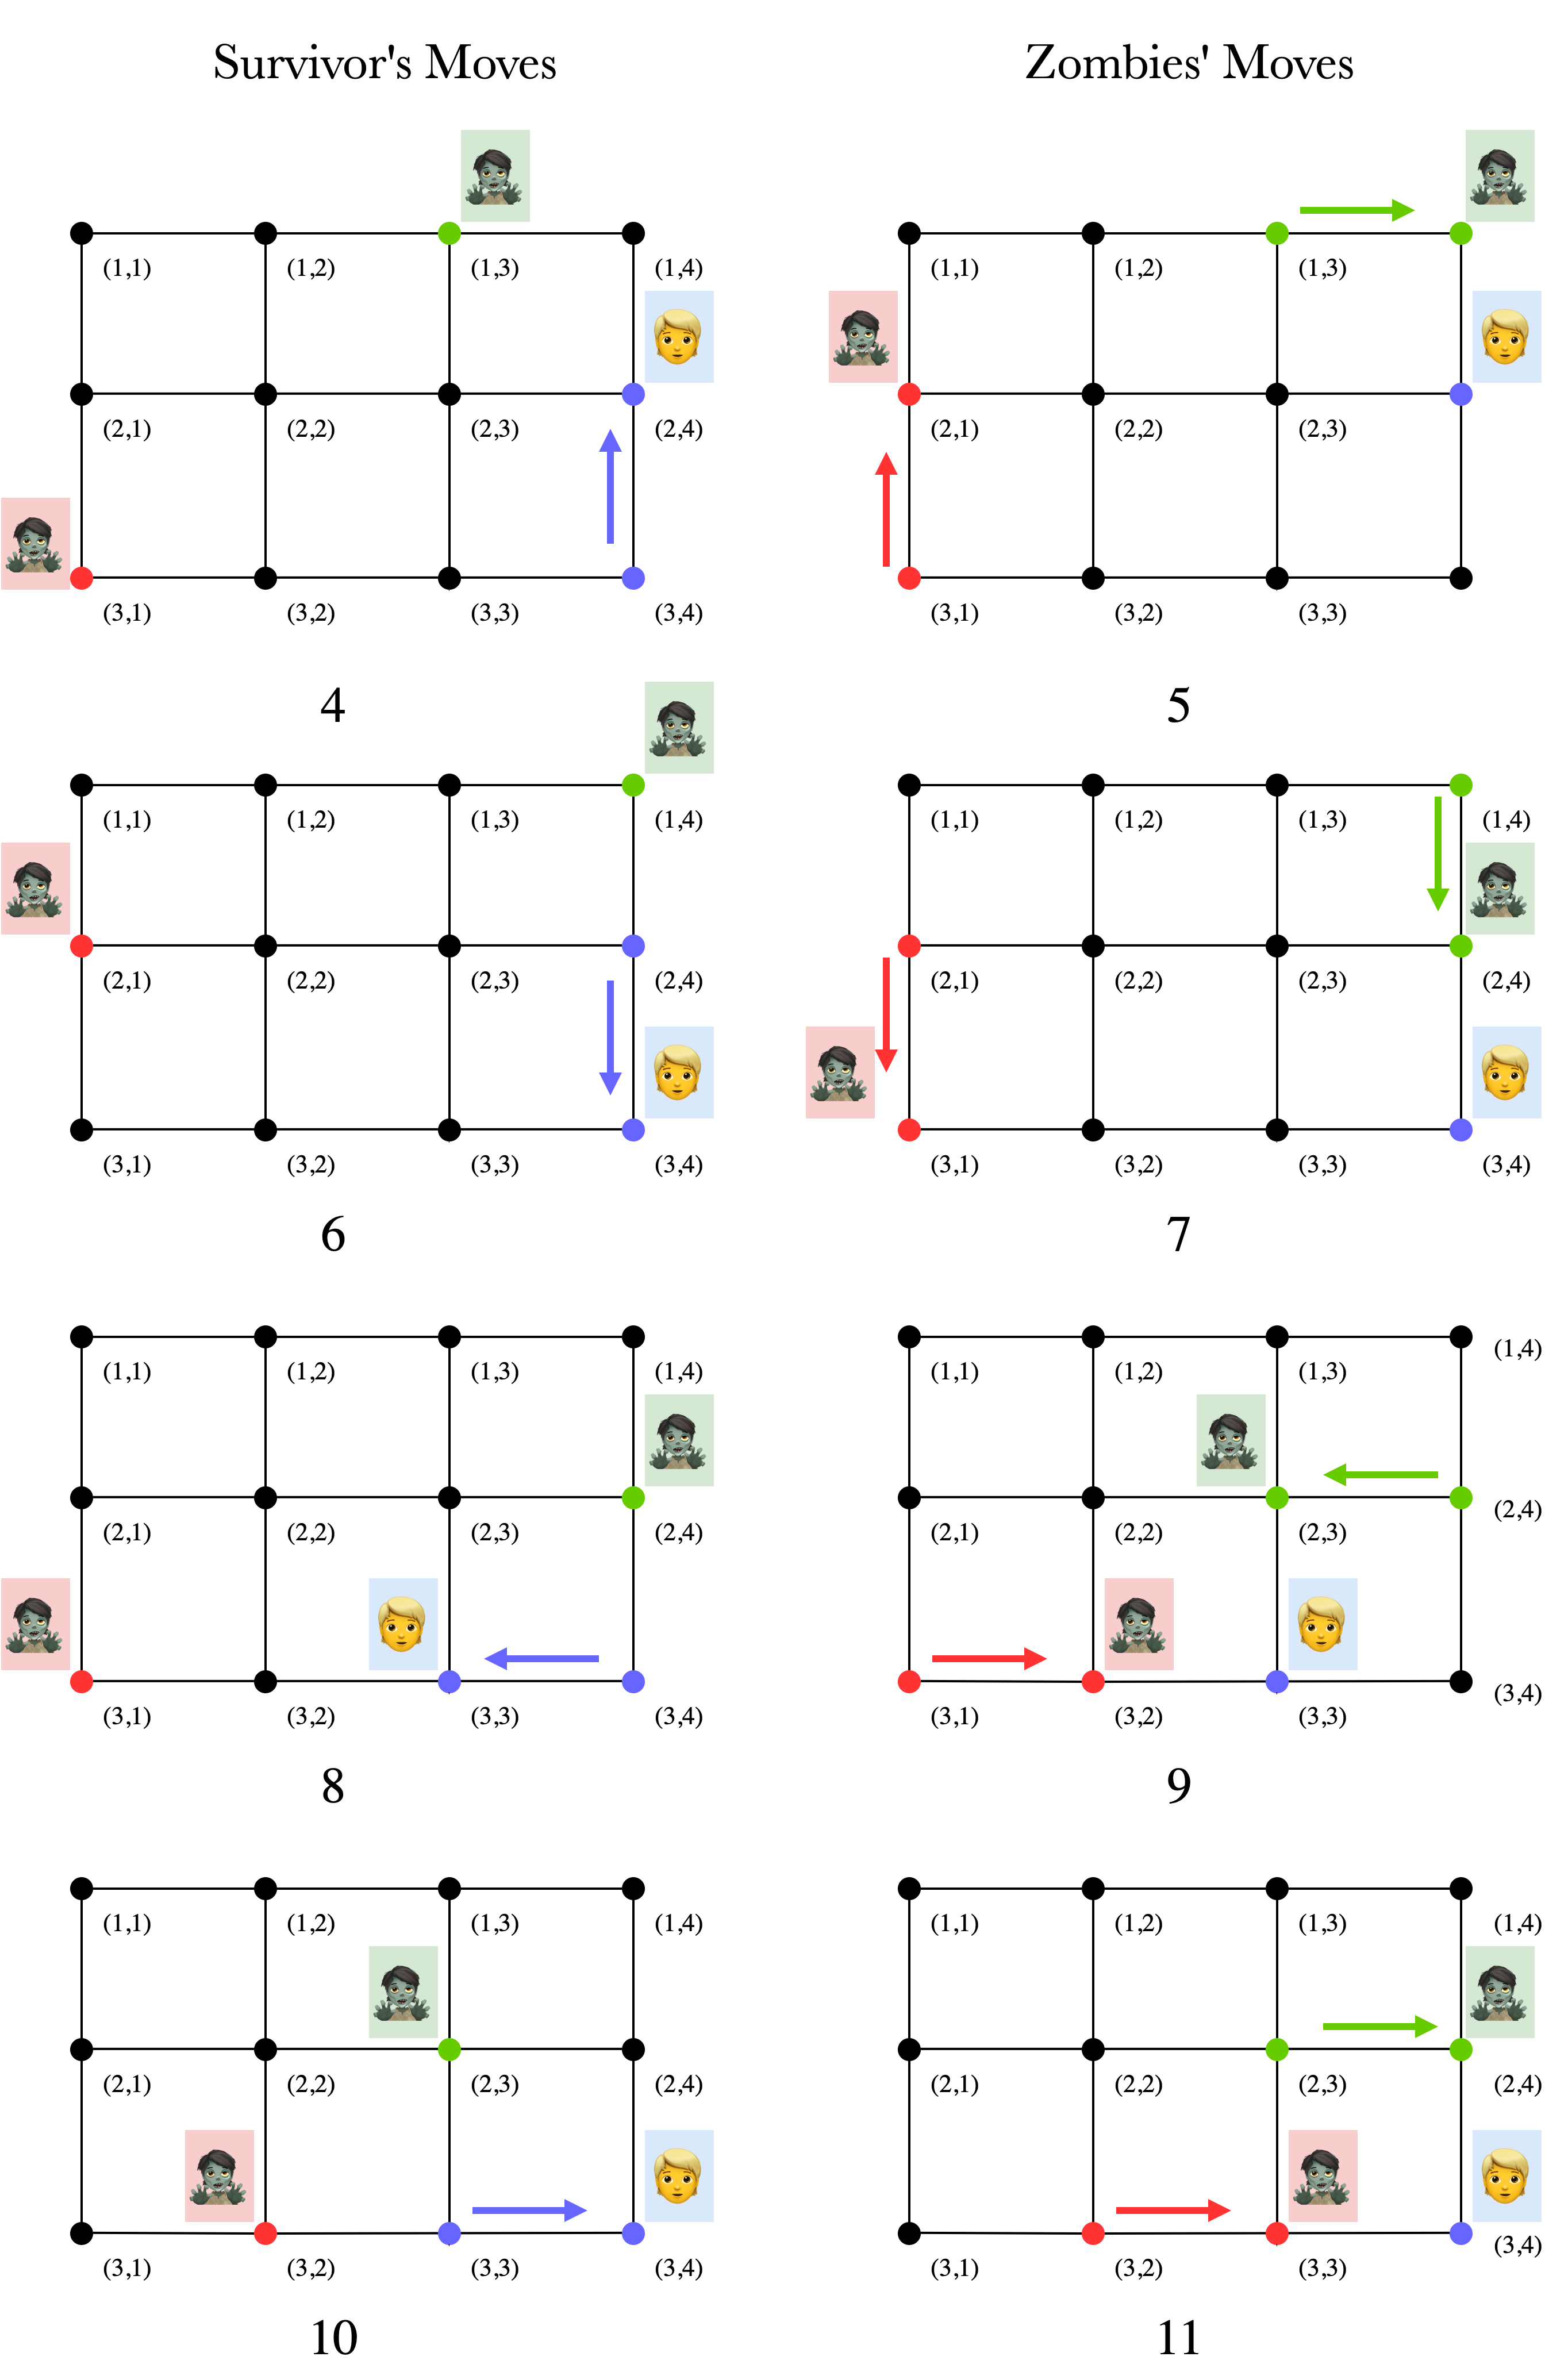
\includegraphics[width=1\linewidth]{p34m6.png}
	\caption{Other moves made by players}
	\label{fig:p6}
\end{figure}

	
\end{document}